%%%%%%%%%%%%%%%%%%%%%%%%%%%%%%%%%%%%%%%%%
% Template para codigo y esas cosas, lo modifique para agregar lo que necesitamos
% Lo afané de:
% http://www.latextemplates.com
%
% Original author:
% Ted Pavlic (http://www.tedpavlic.com)
%
% Me afané la caratula de Algo2 que use el año pasado así nos ahorramos cosas
%
%%%%%%%%%%%%%%%%%%%%%%%%%%%%%%%%%%%%%%%%%

%----------------------------------------------------------------------------------------
%	CONFIG DEL DOCUMENTO Y PAQUETES
%----------------------------------------------------------------------------------------

\documentclass[a4paper,10pt]{article}
\usepackage[paper=a4paper, hmargin=1.5cm, bottom=1.5cm, top=3.5cm]{geometry} % Especifico los margenes a manos
%\usepackage[latin1]{inputenc}	% Codificacion ISO-8859-1
\usepackage[spanish]{babel}
% Colores en los links del índice
\usepackage[colorlinks=true, linkcolor=blue]{hyperref}
\usepackage{courier}
\usepackage{fancyhdr} 		% Custom headers
\usepackage{lastpage} 		% Para obtener la última pagina para el footer
\usepackage{extramarks} 	% Headers y footers
\usepackage[usenames,dvipsnames]{color} % Colores custom
\usepackage{graphicx} 		% Para insertar imagenes
\usepackage{listings} 		% Para insertar codigo
\usepackage{lipsum} 		% 'Lorem ipsum'
\usepackage[section]{placeins}		% Para impedir que las imagenes y eso se vayan a otras secciones que no corresponden
\usepackage{mathtools}
\usepackage{caratula}
%\usepackage[T1]{fontenc}
%\usepackage{algorithmicx, algpseudocode, algorithm}

\hypersetup{%
 % Para que el PDF se abra a pagina completa.
 pdfstartview= {FitH \hypercalcbp{\paperheight-\topmargin-1in-\headheight}},
 pdfauthor={Grupo 25 - Carmen Sandiego, Materia Organizaci\'on del Computador II - DC - UBA},
 pdfkeywords={Informe, TP2, Trabajo, Pr\'actico, II},
 pdftitle={Informe Trabajo Pr\'actico II},
 pdfsubject={Informe Trabajo Pr\'actico II}
}

% Configuración de parrafos
\setlength{\parskip}{1em}


% Margenes
%\topmargin=-0.45in
%\evensidemargin=0in
%\oddsidemargin=0in
%\textwidth=6.5in
%\textheight=9.0in
%\headsep=0.25in

% Line spacing
\linespread{1.1} 

% Set up the header and footer
\pagestyle{fancy}
\lhead{The Mercy Seat} % Header izquierdo
\chead{Informe Trabajo Pr\'actico II} % Header centro
\rhead{\firstxmark Organizaci\'on del Computador II} % Header derecha
\lfoot{\lastxmark}
\cfoot{P\'agina \thepage\ de \protect\pageref{LastPage}} % Footer centro
\rfoot{}
\renewcommand\headrulewidth{0.4pt} % Linea de header
\renewcommand\footrulewidth{0.4pt} % Linea de footer

%\setlength\parindent{0pt} % Remueve identacion de los parrafos

%----------------------------------------------------------------------------------------
%	CONFIGURACION DEL CÓDIGO INCLUIDO
%----------------------------------------------------------------------------------------
\renewcommand{\lstlistingname}{C\'odigo}
\definecolor{DarkGreen}{rgb}{0.0,0.4,0.0} % Comentarios
% Lenguajes soportados: ftp://ftp.tex.ac.uk/tex-archive/macros/latex/contrib/listings/listings.pdf
\lstloadlanguages{[x86masm]Assembler, C} 

%%%%%%%%%%%%%%%%%%%%%%%%%%%%%%%%%%%%%%%%%%%%%%%%%%%%%%%%%%%%%%%%%%%%%%%%%%%%
% Me robe lo de abajo de otro ejemplo, estaba basado en Perl, ver si hay que cambiar algo
\lstdefinestyle{asmStyle}{language=[x86masm]Assembler,
        frame=single,
        breaklines=true, 					% Saltar de linea si supero el maximo
        basicstyle=\small\ttfamily,
        keywordstyle=[1]\color{Blue}\bf,	% Color de las funciones de assembler
        keywordstyle=[2]\color{Purple},		% Color de parámetros especiales (registros, etc)
        identifierstyle=,                               
        commentstyle=\usefont{T1}{pcr}{m}{sl}\color{DarkGreen}\small,
        stringstyle=\color{Purple}, 		% Strings purpuras
        showstringspaces=false,
        tabsize=4,
        %
        % Instrucciones no incluidas en el paquete Assembler
        morekeywords={global, define, section, .rodata, .text, jl, movd, movdqu, mulss, subss, addss, cmpss, pand, cvtss2si, cvttss2si, cvtsi2ss, pxor, pslldq, movq, pshufb, paddb, pmaxub, punpcklbw, punpckhbw},
        %
        % Registros y esas otras cosas especiales que no son instrucciones
        morekeywords=[2]{rax,al,rdx,rcx,rbx,rsi,rdi,rsp,rbp,r8,r9,r10,r11,r12,r13,r14,r15,xmm0,xmm1,xmm2,xmm3,xmm4,xmm5,xmm6,xmm7
        		xmm8,xmm9,xmm10,xmm11,xmm12,xmm13,xmm14,xmm15,r8b, r9b, r10b, r11b, r8d, r9d, r10d, r11d},
        morecomment=[l][\color{Blue}]{...}, % Line continuation (...) like blue comment
        numbers=left,						% Numeros de linea en la izquiera
        firstnumber=1, 						% Se arranca en la linea 1
        numberstyle=\tiny\color{Blue}, 		% Numeros de linea en azul y chicos
        stepnumber=5, 						% Los numerros de linea se muestran cada 5
        numbers=left	                    % where to put the line-numbers; possible values are (none, left, right)
}

%%%%%%%%%%%%%%%%%%%%%%%%%%%%%%%%%%%%%%%%%%%%%%%%%%%%%%%%%%%%%%%%%%%%%%%%%%%%%
% Declaro colores y cosas para C
\lstdefinestyle{cStyle}{language=C,
        frame=single,
        breaklines=true, 					% Saltar de linea si supero el maximo
        basicstyle=\small\ttfamily,
        keywordstyle=[1]\color{Blue}\bf,	% Color de las funciones de assembler
        keywordstyle=[2]\color{Purple},		% Color de parámetros especiales (registros, etc)
        identifierstyle=,                               
        commentstyle=\usefont{T1}{pcr}{m}{sl}\color{DarkGreen}\small,
        stringstyle=\color{Purple}, 		% Strings purpuras
        showstringspaces=false,
        tabsize=4,
        %
        morekeywords={define},
        %
        % Cosas especiales
        morekeywords=[2]{rax},
        morecomment=[l][\color{Blue}]{...}, % Line continuation (...) like blue comment
        numbers=left,						% Numeros de linea en la izquiera
        firstnumber=1, 						% Se arranca en la linea 1
        numberstyle=\tiny\color{Blue}, 		% Numeros de linea en azul y chicos
        stepnumber=2, 						% Los numerros de linea se muestran cada 5
        numbers=left	                    % where to put the line-numbers; possible values are (none, left, right)
}



%%%%%%%%%%%%%%%%%%%%%%%%%%%%%%%%%%%%%%%
% Comando para incluir un archivo de assembler, no hay que poner la extensión
\newcommand{\asmscript}[5]{
\\
\begin{minipage}{\linewidth}
\lstinputlisting[style=asmStyle,caption=#3,label=#1,firstline=#4,lastline=#5]{include/#2.asm}
\end{minipage}
}

% Comando para incluir un archivo C, no hay que poner la extensión
\newcommand{\cscript}[5]{
\\
\begin{minipage}{\linewidth}
\lstinputlisting[style=cStyle,caption=#3,label=#1,firstline=#4,lastline=#5]{include/#2.c}
\end{minipage}
}

\newcommand{\recuadro}[1]{
\noindent\framebox[\columnwidth][c]{\begin{minipage}{0.98\columnwidth}#1\end{minipage}} % Recuadro simple, pongo lo que pasan por parametro
}
%----------------------------------------------------------------------------------------


%----------------------------------------------------------------------------------------
%	ARRANCA EL DOCUMENTO
%----------------------------------------------------------------------------------------
\begin{document}

\materia{Organizaci\'on del Computador II}
\submateria{Segundo Cuatrimestre de 2015}
\titulo{Trabajo Pr\'actico II}
\subtitulo{Informe}
\grupo{The Mercy Seat}

% Puse por orden alfabetico (de nombre), justo queda DFG
\integrante{Christian Murga}{982/12}{christianmmurga@gmail.com}
\integrante{David Ventura}{673/13}{davidventura27@gmail.com}
\integrante{Fabian Alvarez}{674/13}{falvarez.0104@gmail.com}

\maketitle

%----------------------------------------------------------------------------------------
%	TABLE OF CONTENTS
% Hay que compilar dos veces el pdf para que pueda armarla!!!
%----------------------------------------------------------------------------------------

\tableofcontents
\newpage


% Para que no tire conflictos si estamos modificando mucho, separe en distintos archivos el Blur, Merge y HSL
% Si hace falta se pueden separar más. Para compilar se tiene que hacer desde el "informeTP2.tex"

% Para referencias y eso: http://en.wikibooks.org/wiki/LaTeX/Labels_and_Cross-referencing
% ------
% Floatbarrier sirve para que las cosas "flotantes" (imagenes) no se cambien de sección: 
%      http://tex.stackexchange.com/questions/279/how-do-i-ensure-that-figures-appear-in-the-section-theyre-associated-with
%
% --------------------------------------------------------------------------------------------------------------------
% AAAAAAAAAAAAAAAAAAAAAAAAAAAAAAAAAAAAAAAAAAAAAAAAAAAAAAA
% http://www.brendangregg.com/perf.html


% Introducción
\section{Introducci\'on}
El presente informe resume el comportamiento y algoritmos utilizados para la creaci\'on de los filtros de Diferencia de im\'agenes y Blur Gaussiano en sus impelemtaciones en C y Ensamblador, los resultados de los experimentos que se realizaron para evaluar las diferencias entre ambas
implementaciones de los filtros de im\'agenes. As\'i como las conclusiones obtenidas y evidencias de qu\'e cambios podr\'ian mejorar el rendimiento en ciertos casos.

\subsection{Descripci\'on de metodolog\'ia de pruebas}
Las mediciones se realizar\'an mediante un script de python en el cual se ejecuta: \\
\recuadro{\begin{center}\textit{perf stat -B -e cache-references,cache-misses,cycles,instructions}\end{center}}
para cada imagen del conjunto de prueba y para cada par\'ametro de entrada. \\
Esto nos permite, adem\'as de los datos informados por el binario de la c\'atedra, evaluar cantidad de ciclos, instrucciones ejecutadas, estado de cache, etc.

Se planea ejecutar 500 iteraciones de los algoritmos correspondientes, evitando leer/abrir/escribir la imagen en cada iteraci\'on, lo que nos permite medir casi exclusivamente el tiempo de ejecuci\'on del algoritmo. \\
Para eliminar diferencias en los tiempos de ejecuci\'on debido a temas de clock se realizar\'an todas las pruebas en una misma computadora, utilizamdo el governor del procesador en \textbf{performance} y para descartar que procesos en segundo plano alteren los resultados los tests se ejecutar\'an con un par\'ametro \textbf{\textit{nice}} de $-20$. \\
En la secci\'on \ref{sec:specs} se detalla la informaci\'on de la computadora donde se corren los tests y sistema operativo de la misma. \\
Los tests de las implementaci\'on en \emph{C} se corrieron con el nivel de optimizaci\'on "\textbf{-O3}".

En cada prueba particular se definir\'an, si hay, los cambios en las metodolog\'ias de pruebas y se evidenciar\'a con salida de c\'odigo o con diferentes gr\'aficos cuales fueron los resultados obtenidos. \\
Ya que los algoritmos no dependen del contenido de la im\'agen se generaron imagenes aleatorias con la herramienta \textit{imagemagick}.
A partir de las im\'agenes aleatorias se crearon copias de distintos tama\~nos: 16x16 [pixeles], 32x32, 64x64, 256x256 y 1024x1024. \\
Adicionalmente, se crearon algunas im\'agenes de otras dimensiones para evaluar el efecto de ciertas caracter\'isticas en el ejecuci\'on de los algoritmos; por ejemplo, im\'agenes de 128x512 y 512x128 para determinar si la \'unica variable en el tiempo de ejecuci\'on es el tama\~no o si el ancho y el alto (manteniendo una cantidad constante de pixeles) tambi\'en lo afectan.

\subsection{Especificaci\'on t\'ecnica}
\label{sec:specs}
Todas las pruebas las corrimos en la misma computadora, con las siguientes especificaciones
\begin{itemize}
\item Procesador: AMD FX-8350
\item Memoria Ram: 8GB
\item Sistema Operativo: Debian Testing (Linux 4.1.0-2)
\item Governor: Performance
\item 'Niceness' del proceso: -20
\item Archivo de salida: /dev/null
\end{itemize}
\newpage

% Desarrollo
\section{Desarrollo}

% Diff
\subsection{Diferencia de Im\'agenes}
El filtro de diferencias de imagenes consiste en leer dos im\'agenes de iguales dimensiones y computar las diferencias en los p\'ixeles de ambas im\'agenes, analizando los canales (B, G y R) de cada pixel de la primera imagen cotra los del pixel equivalente de la segunda. El canal alpha se ignora y se almacena siempre el valor $255$. En esta implementación de diff, luego de calcular la diferencia de cada canal, se almacena en todos los canales el valor del canal con mayor diferencia. Por ejemplo: \\
$$ Pixel1: |60|80|55|255|$$
$$ Pixel2: |30|88|51|255|$$
$$ Result: |30|30|30|255|$$

\subsubsection{Implementaci\'on C}
\label{sec:diff_impc}
Para mantener m\'as limpio el c\'odigo y facilitar la lectura se cre\'o una funci\'on llamada \textbf{\emph{max}} que devuelve el m\'aximo de 3 valores enteros pasados por par\'ametro. En el c\'odigo \ref{diffc_1} se puede ver la funci\'on creada.\\
%\cscript{diffc_1}{diff_c}{Diff C - Funci\'on de comparaci\'on de valores}{6}{12}

Antes de iniciar el procesamiento se realiza un casteo de los punteros a im\'agenes recibidos para poder operar con los mismos como matrices. Tambi\'en se declaran las variables que se van a usar para recorrer las imagenes y almacenar el valor del diff. \\
Se procede a operar con un ciclo \textbf{\emph{for}} para las columnas y dentro otro ciclo \textbf{\emph{for}} para recorrer las filas, dentro de este \'ultimo ciclo se multiplica la cantidad de filas por $4$ y se incrementa el contador de a $4$ para poder avanzar de a 1 pixel.

Dentro de ambos for se realiza una resta componente a componente de ambos p\'ixeles de ambas im\'agenes, ignorando el canal alpha. A dicho resultado se le calcula el valor absoluto para remover valores negativos y se llama a la funci\'on \emph{max} para obtener la m\'axima diferencia de los 3 componentes, dicho valor se almacena en una variable.

Luego se escribe en la imagen de destino el mismo valor en los 3 componentes del p\'ixel, para que se vea en blanco y negro, y se utiliza el valor 255 para el canal alpha. En el c\'odigo \ref{diffc_2} se puede obvervar como se almacenan los valores en forma secuencial en cada componente, de nota que para escribir en cada canal se suma el offset correspontiente.
%\cscript{diffc_2}{diff_c}{Diff C - Asignaci\'on en destino de cada componente}{28}{31}

~
~

\subsubsection{Implementaci\'on Ensamblador}
\label{sec:diff_impasm}
Esta implementaci\'on, a diferencia de la implementaci\'on en C, se intenta realizar todas las operaciones de forma empaquetada sobre m\'ultiples p\'ixeles a la vez. En la mayor\'ia de las instrucciones se logra operar de a 4 p\'ixeles por instrucci\'on, salvo algunos casos que para evitar problemas de overflow se trabajan con 2.

Antes de iniciar el procesamiento se calcula el tama\~no total de la imagen en \textbf{bytes}, realizando la multiplicaci\'on 
"$filas * columnas * 4$", dicho valor se almacena en un registro de pro\'posito general, el cual se va a usar posteriormente para controlar el recorrido de la imagen. Tambi\'en se limpia un registro para usar de contador y recorrer internamente la imagen.

Para facilitar las cuentas y el procesamiento a futuro se carga en un registro el valor \emph{255} para escribir en el canal alpha y se copia a un registro \emph{XMM}, se realiza un shift del valor para que quede en la posición \textbf{correspondiente al valor alpha del \'ultimo pixel} que se lee en memoria, esto se realiz\'o para que coincida con las m\'ascaras que se pueden ver en el c\'odigo \ref{diffasm_1} \\ 
Duchas m\'ascaras se carga cada uno en un registro \emph{XMM} separado y se realiza un \textbf{xor} de otro registro que va a usarse para desempaquetar los datos.
%\asmscript{diffasm_1}{diff_asm}{Diff ASM - M\'ascaras para realizar shuffle de canales}{14}{23}

En el c\'odigo \ref{diffasm_2} puede observarse como se realiza la carga del valor \emph{255} en el registro \textbf{AL}, luego se pasa al registro \textbf{XMM11} y se realiza el \emph{shift} como el valor especificado en los defines en el c\'odigo \ref{diffasm_1}, as\'i como la carga de las  otras m\'ascaras. \\
%\asmscript{diffasm_2}{diff_asm}{Diff ASM - Carga de valor alpha predefinido}{46}{55}


\textbf{Lectura imagen 1:} \\
Se sabe que al leer de a \emph{Double Quadword} se leen 4 p\'ixeles a la vez. Como el valor de cada p\'ixel se encuentra entre $0$ y $255$, el mismo se almacena en un byte, por lo que cada byte del registro corresponde a un componente del mismo.
$$ XMM0 = |B(P1)|G(P1)|R(P1)|A(P1)|B(P2)|G(P2)|R(P2)|A(P2)|B(P3)|G(P3)|R(P3)|A(P3)|B(P4)|G(P4)|R(P4)|A(P4)| $$
Se lee un \emph{Double Quadword} de memoria en la direcci\'on a la que apunta \emph{RDX} y se almacena en el registro \emph{XMM0}, se realiza una copia del mismo en \emph{XMM1}. De esta forma se cargan de memoria 4 p\'ixeles a la vez. \\
Se procede a desempaquetar los 4 p\'ixeles 2 veces para poder procesar cada uno sin problemas de overflow. Se desempaqueta de \emph{byte} a \emph{word} utilizando las operaciones \textbf{punpck\{l,h\}bw} para las partes altas y bajas respectivamente. De esta forma se almacena en la parte baja (\textbf{XMM0}) los primeros 2 p\'ixeles, siendo cada canal de tama\~no \emph{word} y en el registro \textbf{XMM1} los 2 p\'ixeles correspondientes a la parte alta.

\textbf{Lectura imagen 2:} \\
La lectura y desempaquetado de la imagen 2 se realiza de forma similar a la imagen 1, pero se utiliza como puntero el registro \emph{RCX} y se almacenan los p\'ixeles en otros 2 registros \emph{XMM}. En el c\'odigo \ref{diffasm_3} se puede observar las operaciones de desempaquetado para cada im\'agen. 
%\asmscript{diffasm_3}{diff_asm}{Diff ASM - Lectura y desempaquetado de p\'ixeles}{64}{69}

Se realiza la diferencia de los p\'ixeles de cada imagen componente a componente. Como se realiz\'o el desempaquetado del mismo modo, los p\'ixeles quedar\'an alineados con su contraparte en la otra imagen. Como esta operaci\'on puede dar valores negativos, se utiliza la instrucci\'on \textbf{pabsw} para obtener el valor absoluto de dicha diferencia.
Como se sabe que luego de realizar la diferencia y calcular el valor absoluto, cada canal no puede valer m\'as de $255$, se empaquetan nuevamente como \emph{Byte} saturados sin signo los registros de destino utilizados en la instrucci\'on anterior, con esto se finalizar\'ia el c\'alculo del la diferencia y se procede a calcular el valor m\'aximo.

Como la diferencia en los canales alpha va a dar siempre $0$ para las im\'agenes que se procesan, antes de aplicar los \textbf{shuffle} se suma al registro que va a almacenar el canal \textbf{azul} el registro especial con el valor de alpha calculado al comienzo del procesamiento, esto dejaría el registro de la siguiente manera:
$$ XMM0 = |VAL|VAL|VAL|0|VAL|VAL|VAL|0|VAL|VAL|VAL|0|VAL|VAL|VAL|255| $$
donde \emph{VAL} es un n\'umero entre $0$ y $255$. Al momento de utilizar el \textbf{shuffle} al canal azul se copiar\'an los valores de alpha en todos canales alpha de los p\'ixeles. Como los valores de alpha de los otros canales pueden ser menores o iguales a $255$, me aseguro que al calcular el mayor va a quedar dicho valor. \\
La l\'ogica del c\'alculo del valor m\'aximo consiste en utilizar las 3 m\'ascaras, para los canales \textbf{B}, \textbf{G} y \textbf{R}, para realizar un \textbf{shuffle} a byte. Dichas m\'ascaras se encargan de repetir el valor que corresponde (componente B, G o R) en todos los canales de cada p\'ixel. Se utiliza un registro \textbf{XMM} auxiliar para cada m\'ascara. Por ejemplo, si se tiene el siguiente registro:
$$ XMM0 = |99|5|5|255|42|0|0|255|......| $$
al aplicar la m\'ascara \textbf{BLUE\_MASK} se obtendr\'ia: \\
$$ XMM0 = |99|99|99|255|42|42|42|255|......| $$
Dicha operaci\'on se realiza para cada componente en los registros auxiliares y luego se obtiene el m\'aximo canal de los 3 registros utilizando la instrucci\'on \emph{pmaxub}. \\
En  el c\'odigo \ref{diffasm_4} se puede observar las intrucciones para procesar todos los canales.
%\asmscript{diffasm_4}{diff_asm}{Diff ASM - Aplicaci\'on de m\'ascaras y c\'alculo de maximo canal}{77}{85}

Para finalizar se escriben los 4 p\'ixeles en memoria, se avanzan los punteros enteros en \emph{16 bytes} y se repite el ciclo hasta que no haya p\'ixeles por procesar.


\subsubsection{Hip\'otesis de funcionamiento para los experimentos}
Con saber el funcionamiento de los algoritmos se pueden realizar algunas especulaciones respecto al funcionamiento del programa, tales como: \\
En la implementaci\'on en ASM se podr\'ia esperar una clara mejora de performance en cuanto a la implementaci\'on secuencial de C, ya que hay hasta $4$ veces menos lecturas y escrituras a memoria. La forma de ejecuci\'on de datos empaquetados tambi\'en puede influir en que se consumen menos ciclos de reloj y movimientos de datos. \\
Otro factor que podr\'ia influir en menor medida es que en la implementaci\'on \textbf{C} el m\'aximo valor se calcula en una funci\'on separada, para la cual se tiene que armar su stack frame y realizar varios saltos condicionales y saltar nuevamente al ciclo principal de procesamiento, todo esto para cada p\'ixe que se procese, mientras que para la implementaci\'on \textbf{ASM} el m\'aximo se calcula con aproximadamente $2$ instrucciones para cada p\'ixel, todas operando dir\'ectamente con registros y no accediendo a memoria. Para comprobar este caso se puede declarar la funci\'on en C con un \emph{inline}.

\newpage

% Blur Gaussiano
\subsection{Blur Gaussiano}
El filtro Blur Gaussiano consiste en, dado un radio \textbf{r} y un par\'ametro $\sigma$, \emph{generar} una matriz de convoluci\'on, la cual no depende de los valores de la imagen, por lo que puede ser calculada una sola vez. Luego con esa matriz se toma una \emph{sub-matriz} de radio \textbf{r} con centro en el p\'ixel que se quiere procesar y realizar una sumatoria de la multiplicaci\'on componente a componente de cada matriz. Esto resulta en una imagen m\'as "borrosa" (a lo que se debe el nombre del filtro).

\subsubsection{Implementaci\'on C}
\label{sec:blur_impc}
Para simplificar el c\'odigo en \textbf{C} y \textbf{ASM} se cre\'o  una funci\'on encargada de calcular la matriz de convoluci\'on. La matriz se almacena en el heap y se devuelve un puntero a la misma para realizar los c\'alculos. Queda a cargo del c\'odigo que utilice a dicha matriz llamar al \emph{free} para liberar la memoria.
Para generar la matriz primeramente se calcula el largo de la misma, el cual es $(2*r + 1)^2$, al momento de llamar a la funci\'on \textbf{malloc} se multiplica dicho valor por el tama\~no de un float. \\
Luego se realizan dos ciclos \textbf{\emph{for}} anidados, uno para recorrer las columnas y otro para recorrer las filas. Los valores van desde $-r$ a $r$. Para cada elemento realizo la ecuaci\'on gaussiana en dos dimensiones y lo almaceno en la matriz. \\
Al finalizar queda la matriz de convoluci\'on con \emph{float}, donde cada elemento de la matriz corresponder\'ia a un p\'ixel. \\
En el c\'odigo \ref{blurc_1} se puede ver el ejemplo del código que se ejecuta.
%\cscript{blurc_1}{blur_c}{Blur C - Ciclo princip\'al de calculo de matriz de convoluci\'on}{24}{36}

Antes de iniciar el procesamiento se realiza un casteo de los punteros a im\'agenes recibidos para poder operar con los mismos como matrices. Tambi\'en se declaran las variables que se van a usar para recorrer la imagen y la sub-matriz. Se llama a la funci\'on para obtener la matriz de convoluci\'on y se almacena el puntero a la misma.\\
Se procede a recorrer la imagen con dos ciclos \textbf{\emph{for}} anidados, los mismos van desde \emph{Radio} hasta $Filas-Radio"$ y $Columnas-Radio$, esto produce que no se recorran ni procecen los bordes de la im\'agen.
Dentro del ciclo interno se reinicia (asigna $0$) al acumulador interno, se reinicia tambi\'en el contador de posici\'on de la matriz de convoluci\'on.

\emph{NOTA: Descubrimos que el puntero de destino tiene el mismo contenido que la imagen de origen, esa es la raz\'on por la que no leemos ni escribimos en los bordes. Si llegara a cambiar esto, deber\'ia añadirse un bloque peque\~no de c\'odigo que copie los bordesde de tama\~no $Radio$ de la im\'agen de origen sin procesarlos.}

Para cada ciclo interno, luego de reiniciars las variables se realizan otros dos ciclos \textbf{\emph{for}} anidados para calcular la sumatoria de la sub-matriz que le corresponde al p\'ixel actual. Dichos ciclos van, al igual que los ciclos que se usan para calcular la matriz de convoluci\'on, desde $-Radio$ hasta $Radio$.\\
Luego se multiplica cada componente del p\'ixel que se recorre por la matriz de convoluci\'on en la misma posici\'on, se almacena en el acumulador y antes de terminar el ciclo se aumenta la posici\'on de la matriz de convoluci\'on. Esta operaci\'on se realiza por cada elemento de la sub-matriz (por los ciclos \emph{for}).

Al finalizar la sumatoria de la sub-matriz se guardan los valores de la sumatoria en cada canal del pixel actual en la imagen de destino y se contin\'ua con el ciclo. En el c\'odigo \ref{blurc_2} puede verse la operaci\'on de almacenamiento de cada componente en la imagen de destino.
%\cscript{blurc_2}{blur_c}{Blur C - Ciclo princip\'al de calculo de matriz de convoluci\'on}{61}{64}
Luego de finalizado el ciclo principal se procede a llamar a la funci\'on \textbf{free} y liberar la memoria utilizada por la matriz de convoluci\'on.


\subsubsection{Implementaci\'on Ensamblador}
\label{sec:blur_impasm}

Para minimizar confusion renombramos los registros \\
%\asmscript{Defines}{blur_asm}{Define}{9}{22}

Al iniciar el filtro, se \emph{pushean} los registros \emph{XMM0,src,dst,cols,filas,radius}, para resguardarlos al llamar a convolucion\_matrix, el resultado de esta funcion se guarda en \emph{matriz y r15} \\
Calculamos el tama\-no correspondiente de la imagen en bytes(ancho) o pixeles(alto) y luego avanzamos \emph{radius} filas para no tener en cuenta los bordes; tambien los restamos del alto y ancho total de la imagen. \\
El recorrido de la imagen se hace iterando a traves de cada fila de la imagen ( \emph{cols-2*radius pixeles} ), un total de \emph{filas-2radius} veces. \\
Al inicio del recorrido de cada fila, avanzamos \emph{src} y \emph{dst} en \emph{radius} pixeles, siendo estos el borde.  \\
Una vez posicionados sobre un pixel no-borde procedemos a iterar por la matriz de convoluci\'on, esto se hace llevando la cuenta de filas y columnas restantes para terminar (sabiendo que inicialmente estas valen \emph{2*radius+1}). \\
El procesamiento de dentro de la matriz de convoluci\'on es el siguiente:
\begin{itemize}
\item Leer 16 bytes de memoria desde src*
\item Eliminar los pixeles ya procesados*
\item Desempaquetar los pixeles, en un registro cada uno
\item Leer 16 bytes de memoria desde matriz*
\item Acomodar estos factores de forma que podamos multiplicarlos elemento a elemento con los pixeles
\item Convertir los pixeles a punto flotante y multiplicarlos por los factores
\item Acumular los productos
\end{itemize}

*Nunca leemos fuera de la memoria asignada, porque en caso de que nos queden menos de 16 bytes por leer, retrocedemos esta diferencia en los punteros y luego volvemos cero a los factores repetidos para evitar a\-nadirlos dos veces al resultado. \\
%\asmscript{Retroceso}{blur_asm}{Retroceso}{185}{188}

Una vez que, para un pixel dado, recorremos completamente la matriz de convolucion, guardamos el resultado acumulado y avanzamos los punteros \emph{src y dst}. Seguimos iterando hasta recorrer la imagen de forma completa.
\newpage

% Conclusion
\section{Resultados}
\FloatBarrier
\subsection{Blur Gaussiano}

La l\'ogica de procesamiento de ambas implementaciones del blur \textbf{no} depende del tipo de im\'agenes, por lo que se procedi\'o a realizar unas pruebas preliminares con distintas imagenes aleatorias y mon\'ocromas. Los tiempos de ejecuci\'on de dichas imagenes resulto ser similar, habiendo peque\~nas diferencias aleatorias que se relacionaron con otras actividades que pudo haber estado realizando el sistema operativo. Por lo que se eligi\'o una de esas im\'agenes al azar para realizar el resto de las pruebas.

Se pudo observar que al realizar el procesamiento con valores de radio chicos (no mayor a 3) los tiempos de ejecuci\'on son similares, esto se asocia al calculo adicion\'al que realiza la implementaci\'on en \textbf{Ensamblador} al momento de procesar las \'ultimas columnas de la sub-matriz se vuelven a procesar reiteradas veces algunos p\'ixeles, pero m\'as que nada se tienen muchos saltos condicionales para no realizar lecturas inv\'alidas. En radios gr\'andes grandes ese procesamiento repetido se vuelve despreciable y se puede apreciar la ganancia de velocidad al realizar muchas menos operaciones de lectura en la implementaci\'on en \textbf{Ensamblador}.
Observamos que, como se hace el c\'alculo de la matriz de convoluci\'on en \textbf{C}, esto tambi\'en puede condicionar un poco los tiempos de ejecuci\'on con imagenes con radio peque\~no, en im\'agnes con radio grande, nuevamente, este valor empieza a tornarse despreciable.

En un principio resulta extra\~no el comportamiento de la implementaci\'on \emph{Ensamblador} con im\'agenes peque\~nas, en la cual los tiempos dieron similares a los de la implementaci\'on \emph{C}, aunque la misma realiza menos lecturas de memoria. Deducimos, entonces, que debido a la cantidad de saltos condicionales que posee dicha implementaci\'on el procesador no puede realizar un manejo de prefetch \'optimo, provocando m\'as estados de espera. Mientras que en la implementaci\'on \emph{C} el compilador realiza optimizaciones y el procesamiento es m\'as secuencial, lo que puede aumentar su performance.

En el resto de los casos el comportamiento es el esperado y solo var\'ia en funci\'on del tamaño de la imagen y del radio. Se conjetura entonces que el rendimiento de los algoritmos est\'a ligado fuertemente a la cantidad de lecturas de memoria, y muy a la cantidad de saltos condicionales en medio del procesamiento.

No se encontr\'o diferencias en los tiempos de procesamiento al cambiar los valores de $\sigma$, esto puede demostrarse por que se utiliza solamente para hacer c\'alculos de la matriz de convoluci\'on, pero no hay saltos ni cambios de l\'ogica que dependan del mismo.

En la figura \ref{fig:figure_blur} se puede observar los resultados de las pruebas realizadas con los diferentes tama\~nos de radio. En los cuales baja el rendimiento con radios peque\~nos (\emph{ASM-S})

%\begin{figure}[htpb]
%    \centering
%    \caption{Tiempo de ejecuci\'on de im\'agenes arbitrarias para el filtro blur con valores arbitrarios }
%    \label{fig:figure_blur}
%    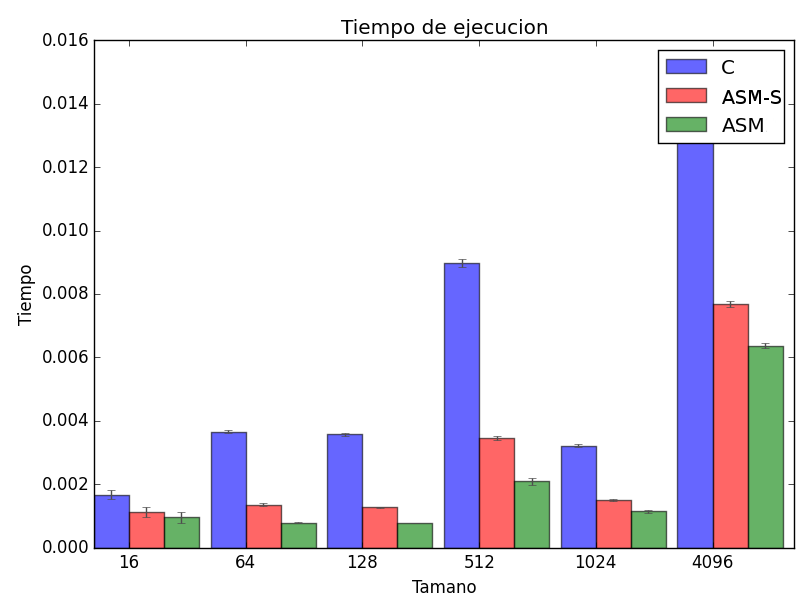
\includegraphics[width=0.75\columnwidth]{include/figure_blur}
%\end{figure}

\FloatBarrier
\subsection{Diferencia de Im\'agenes}

En la primera prueba, para poder notar diferencias significativas. Se ejecut\'o 500 veces cada implementaci\'on del filtro, de esta manera se evita cargar nuevas instancias de los programas y calcular un tiempo incorrecto debido a la carga de d\'isco de las im\'agenes, cache de disco, la invocaci\'on de tareas, y se puede evaluar el uso de cache.

Se utilizaron im\'agenes de diferentes tama\~nos para simular distintos casos y estudiar el comportamiento del filtro. Como el filtro no consiste, ni tiene l\'ogica que dependa del tipo de im\'agen (aleatoria, alto contraste, etc) nos basamos espec\'ificamente en tama\~nos. \\
Cada prueba se ejecut\'o 10 veces, cada una de estas veces se aplic\'o 500 veces el filtro, y se calcul\'o el promedio para el gr\'afico y la desviaci\'on est\'andar que se obtuvo.

En la figura \ref{fig:figure_blur} se puede observar los tiempos y resultados. Se pueden ver los resultados utilizando el \emph{max} inline, que mejora pero muy poco.

%\begin{figure}[htpb]
%    \centering
%    \caption{Tiempo de ejecuci\'on de im\'agenes arbitrarias, para el filtro diff }
%    \label{fig:figure_diff}
%    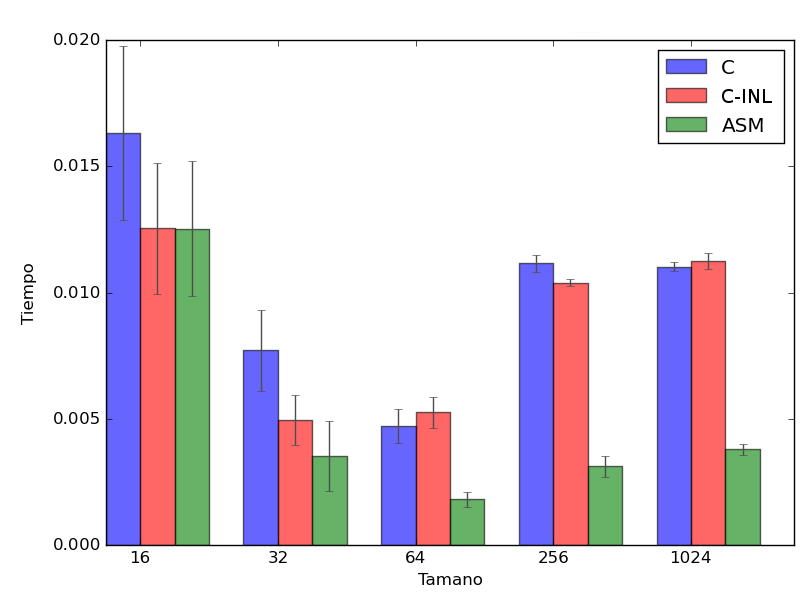
\includegraphics[width=0.75\columnwidth]{include/figure_diff}
%\end{figure}

En la mayor\'ia de los casos los cache-references rondaban el $75.0\%$ mientras que los cache-mises se mantenian menores a $0.05\%$. \\
Puede observarse lo que se hab\'ia predecido en la hip\'otesis, que los tiempos de ejecuci\'on comparados a la implementaci\'on \emph{C} son mucho menores que los tiempos de \emph{Ensamblador}, seguramente debido a la menor cantidad de lecturas de memoria. \\
Tambi\'en se puede conjeturar que influye altamente la cantidad de saltos condicionales y lecturas extras que tiene la implementaci\'on \emph{C} al llamar a la funci\'on \emph{max}.

%TODO CORRER TESTS CON INLINE

Se vi\'o que el tiempo de ejecuci\'on en una imagen de $512x512$ es mucho mayor que $1024x1024$, en especial en la implementaci\'on en C, viendo los datos del cache no pudimos llegar a la conclusi\'on de por que puede funcionar mas lento, ya que los valores son normales y consistentes con las imagenes de $128x128$ y $1024x1024$.


\newpage

% Conclusion
\section{Conclusi\'on}
Se observ\'o que para el filtro Diferencia de im\'agenes, el tiempo de ejecuci\'on de los algoritmos variaba de forma similar al modificar el tama\~no de la imagen de entrada. Adem\'as se not\'o que las proporciones de la imagen no ten\'ian un impacto significativo al modificarse las proporciones (pero manteniendo constante la cantidad total de p\'ixeles). Finalmente, conjeturamos que la superior eficacia del algoritmo C se debe a una mejor econom\'ia de m\'ascaras y uso \'optimo de los registros que permite realizar menos accesos a memoria y menos saltos condicionales.

Como conclusi\'on se conjetura en los casos del Blur Gaussiano, que aunque la lectura es lo que m\'as perjudica el rendimiento, los saltos condicionales pueden causar una gr\'an p\'erdida de rendimiento. \\
Pero en procesamientos con radio chico, la cantidad elevada de saltos condicionales a verificar con la implementaci\'on en \emph{Ensamblador} puede perjudicar el performance, pero cuando se aumenta el tama\~no del radio estas verificaciones se tornan pr\'acticamente despreciables y se puede ver un aumento sustanci\'an en los tiempos de ejecuci\'on del algoritmo.

\pagebreak


\newpage

\end{document}
